\documentclass[8pt]{beamer}

%\useoutertheme[subsection=false]{miniframes}
\usetheme{Singapore}
\setbeamertemplate{frametitle}[default][center]

\usepackage[utf8]{inputenc}
\usepackage{mathtools}
\usepackage{amssymb}
\usepackage{tabularx}
\usepackage{tabulary}
\usepackage{booktabs} % for toprule
\usepackage{xcolor} %to color text
\usepackage[ruled,vlined]{algorithm2e}
\SetAlCapFnt{\small}
\SetAlCapNameFnt{\small}
\usepackage{graphicx}
\usepackage{array}
\usepackage{multirow}
\usepackage{amsmath}
\usepackage[skip=1ex]{caption}
\usepackage{empheq}
\usepackage{fixmath}
\usepackage{comment}
\renewcommand{\thealgocf}{}
\setbeamertemplate{caption}[numbered]

\newcommand\Fontvi{\fontsize{6}{7.2}\selectfont}
\newcommand\Fontli{\fontsize{7}{7.2}\selectfont}
\newcommand{\norm}[1]{\left\lVert#1\right\rVert} %adjust norm sizes
\definecolor{bluepurp}{RGB}{53,44,179}

\beamertemplatenavigationsymbolsempty

\setbeamertemplate{blocks}[rounded][shadow=true]
\definecolor{babyblue}{RGB}{214, 214, 240}
\setbeamercolor{block title}{bg=babyblue}
\setbeamercolor{block body}{bg=normal text.bg!90!white}
\usepackage{dsfont}

\setbeamertemplate{footline}[text line]{
\parbox{\linewidth}{\vspace*{-8pt}\hfill\insertframenumber{} / \inserttotalframenumber}}

\title{Partial Outer Convexification for Compressor Cost Optimization in a Gas-to-Power Network}
\subtitle{Final presentation of Master Thesis}
\institute 
{
Chair of Scientific Computing\\
University of Mannheim
}

\author{Katharina Enin}
\date{02.12.2021}

\begin{document}
\begin{frame}
	\titlepage 
\end{frame}
	
\begin{frame}
\textcolor{orange}{Table of Contents:}
\begin{enumerate}
\item  Introduction
\item Partial Outer Convexification and the Three-Step Approach
\item Physical Characterististics of Gas-to-Power Network
\item Optimization Model
\item Numerical Analysis
\item Conclusion
\end{enumerate}
\end{frame}

\section{Introduction}
\begin{frame}{Goal of the Thesis}
\textcolor{bluepurp}{Goal:} Optimize compressor costs in a Gas-to-Power network.  \newline\newline
\textcolor{bluepurp}{Methods:} We will compare the \textcolor{orange}{three-step approach} based on \textcolor{orange}{Partial Outer Convexification (POC) Reformulation} and the \textcolor{orange}{direct solver Bonmin} working with an NLP-based Branch-and-Bound Algorithm. 
\end{frame}

\section{Three-Step Approach}
\begin{frame}{Three-Step Approach}
\begin{figure}
\centering
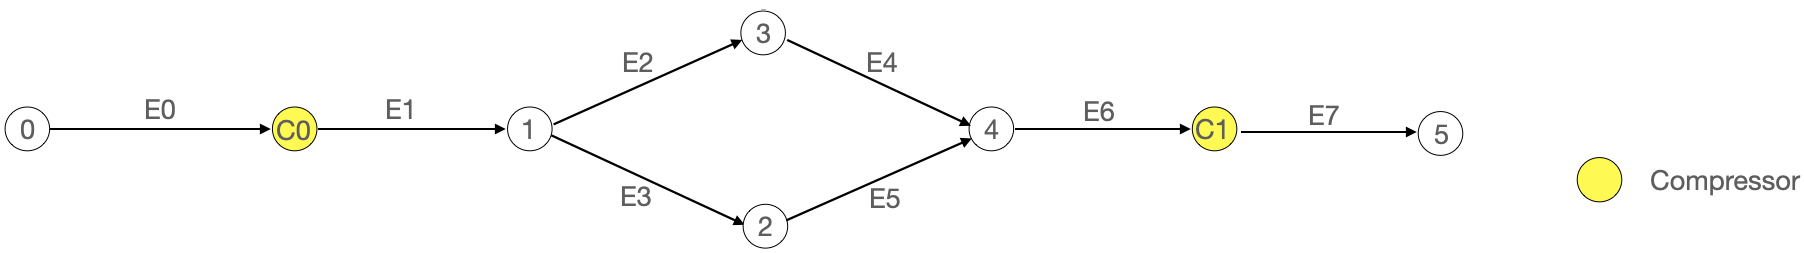
\includegraphics[width=0.7\textwidth]{images/AdvancedNetwork2.png}
\caption{Gas Network}
\end{figure}
In this gas-network we have \textcolor{orange}{two compressors} and \textcolor{orange}{four compressor combinations}
\begin{itemize}
\item compressor 0 is \textbf{off} and  compressor 1 is \textbf{off}: (0,0)
\item compressor 0 is \textbf{off}  and  compressor 1 is \textbf{on}: (0,1)
\item compressor 0 is \textbf{on}  and  compressor 1 is \textbf{off}: (1,0)
\item compressor 0 is \textbf{on}  and  compressor 1 is \textbf{on} : (1,1)
\end{itemize} 
If $n_{com}$ denotes the number of compressors, we have \textcolor{orange}{$n_{oc}= 2^{n_{com}}$} number of combinations. \newline
We introduce \textcolor{orange}{convex multiplier controls} $w^t \in \{0,1\}^{n_{oc}}$ that tell which combination holds in $t$:  e.g. if combination $(0,1)$ in $t$ holds,  then $w_1^t=1$ and $w_k^t=0$ for $k \neq 1$. 
\end{frame}

\begin{frame}{Three-Step Approach}
\Fontli
\textcolor{bluepurp}{1. Formulate Problem into the form \textcolor{orange}{(POC formulation)}:}
\begin{alignat}{2}
\min_{u^t}   \quad & f(x^t,u^t) \label{eq:3.0} & \\
\text{subject to: } 
\quad & x^{t+1} = x^t + \Delta t \Phi(x^t,u^t) \begingroup\color{orange} w^t \label{eq:3.1} \endgroup &\text{(PDE)}\\
& \begingroup\color{orange}\sum_{s=1}^{n_{oc}} w_s^t = 1 \endgroup \text{ with } w^t \in \{0,1\}^{n_{oc}} &\text{(SOS1)} \label{eq:3.2} \\
& \text{( + some additional constraints for $x$, $u$ and $w$)} & \label{eq:3.3}
\end{alignat}
\newline
\textcolor{bluepurp}{2. Apply the following Algorithm:}
\begin{algorithm}[H]
Discretize problem \ref{eq:3.0} - \ref{eq:3.3} with appropriate step sizes $\Delta t$ and $\Delta x$ fulfilling the CFL-condition.\\
\textbf{Step 1}: Relax the integrality conditions 
\begin{equation}
w_s^t \in \{0,1\} \rightarrow \tilde{w}_s^t \in [0,1],  \forall t \in \{0,...,n_T\}, \;\forall s \in \{0,...,n_{oc}\}
\end{equation}
and solve the arising continuous NLP.  This yields the optimal vector $\tilde{w}$.
 \\
\textbf{Step 2}: Compute a feasible binary solution $w$ out of $\tilde{w}$ by solving CIAP (Combinatorial Integral Approximation Problem).\\
\textbf{Step 3}: Simulate the dynamics again with $w$ to obtain a feasible trajectory and a corresponding objective value.  
\caption{Three-Step Approach}
\end{algorithm}
\end{frame}

\begin{frame}{Approximation Theorem for POC}
\Fontvi
\begin{theorem} []
Let $\mathcal{I}  = \{0,...,n_T-1\}$,  $\mathcal{D} \subseteq \mathbb{R}^N$ and $\Phi: \mathcal{I} \times \mathcal{D} \rightarrow \mathbb{R}^{n \times n_{oc}}$ be a matrix-valued function that is continuous with respect to the second argument and satisfies
\begin{alignat}{2}
\| \Phi(t,\mu) \nu \|_X &\leq M_{oc} \|\nu \|_{\Omega}, &\quad \forall t \in \mathcal{I},  \mu \in \mathcal{D}, \nu \in \mathbb{R}^{n_{oc}} \\
\| (\Phi(t,\mu) -\Phi(t,\eta)) \alpha \|_X &\leq L_{oc} \| \mu - \eta \|_{X}, &\quad \forall t \in \mathcal{I}, \mu, \eta \in \mathcal{D}, \alpha \in H 
\end{alignat}
for constants $M_{oc}, L_{oc} < \infty$.  Furthermore,  for each $t \in \mathcal{I}$ let $h_t >0$,  $\alpha^t$,   $\beta^t \in H$ such that $T = \sum_{t=0}^{n_T - 1} h_t$ and for each $t \in \mathcal{I} \cup \{n_T\}$ let $\mu^t,  \eta^t \in \mathcal{D}$ be given such that for all $t \in \mathcal{I}$ 
\begin{equation}
\mu^{t+1} = \mu^t + h_t\Phi(t,\mu^t)\alpha^t  \quad \textrm{and} \quad \eta^{t+1} = \eta^t + h_t\Phi(t,\eta^t)\beta^t.
\end{equation}
If for some set $\mathcal{I}' \subseteq \mathcal{I}$, constants $C_{oc}, \epsilon < \infty$ and some vector $\delta^0 \in \mathbb{R}^{n_{oc}}$ it holds that 
\begin{alignat}{2}
\| (\Phi(t+1,\mu^{t+1}) - \Phi(t, \mu^t)) \nu \|_X &\leq h_t C_{oc} \| \nu \|_{\Omega},  \quad &\forall t \in \mathcal{I}', \nu \in \mathbb{R}^{n_{oc}} \\
\| \delta^0 + \sum_{t=0}^{k-1} h_t(\alpha^t - \beta^t) \|_{\Omega} &\leq \textcolor{red}{\epsilon}, \quad &\forall k \in  \mathcal{I} \cup \{n_T\} 
\end{alignat}
then it follows with $T_k' = k\, max\{h_t | t=0,...,k-1\}$ and $n_{jump} = | \mathcal{I} \setminus (\mathcal{I}' \cup \{n_T - 1\}) |$ that for all $k \in \mathcal{I} \cup \{n_T\}$
\begin{equation}
\sum_{t=0}^k h_t \| \mu^t - \eta^t\|_X \leq \frac{exp(T_k' L_{oc})-1}{L_{oc}}(\| \mu^0 - \eta^0\|_X + (2M_{oc}(1+n_{jump}) +TC_{oc})\textcolor{red}{\epsilon}). 
\end{equation}
\end{theorem}
\end{frame}
\begin{frame}{Step 2: CIAP (General)}
CIAP is denoted as follows: 
\begin{alignat}{1}
\begin{split}
\min_{\substack{\beta^t \in H \cap \{0,1\}^{n_{oc}},  \\ t =0,...,n_T-1,  \\ \delta^0 \in \mathbb{R}^{n_{oc}},\epsilon \in \mathbb{R}_{\geq 0}}}  &\epsilon      \\
\text{subject to: } \quad &\norm{\delta^0 + \sum_{t=0}^{k-1} \Delta t (\alpha^t-\beta^t)}_{\Omega} \leq \epsilon \quad  \text{for all } k=0,...,n_T
\label{Eq:2.1}
\end{split}
\end{alignat}
\textcolor{orange}{Without additional constraints:} Solve with \textbf{Sum Up Rounding (SUR)} \newline
SUR can be solved in polynomial time and its objective value $\epsilon$ is proportional to $\Delta t$
\newline\newline
\textcolor{orange}{With additional constraints that couple over time:} \newline Solve MILP: (\ref{Eq:2.1}) + additional constraints \newline
$\epsilon$ cannot be driven to zero by decreasing $\Delta t$
\end{frame}

\section{GtP Characteristics}
\begin{frame}{Power Network (1)}
\Fontli
\begin{figure}[l]
\centering
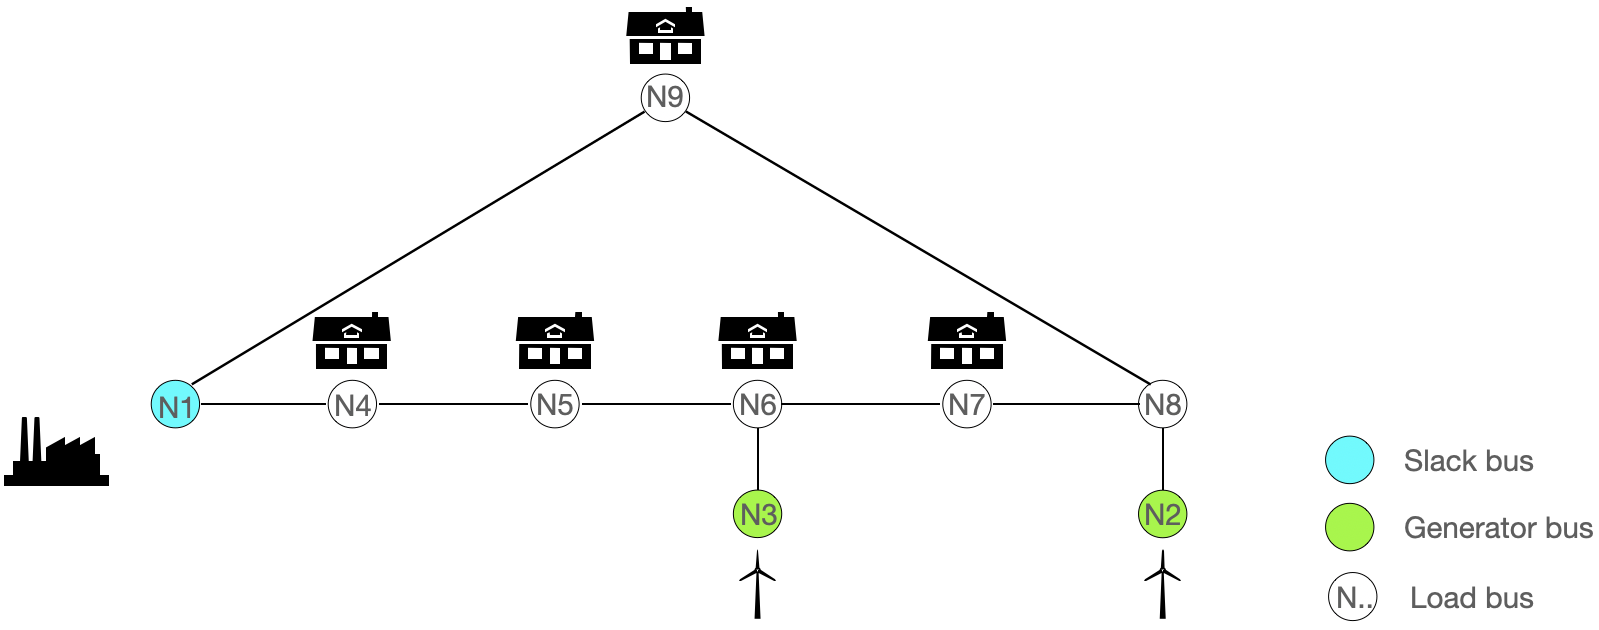
\includegraphics[width=0.6\textwidth]{images/PowerNetwork}
\caption{Power Network with one slack bus, two generator buses and six load buses}
\label{PG}
\end{figure}
\textcolor{bluepurp}{Power Flow Equations:}
\begin{alignat}{2}
\begin{split}
P_k &= \sum_{j=1}^N |V_k| |V_j| (G_{kj}cos(\phi_{k,j})+B_{kj}sin(\phi_{k,j})) \\
Q_k &= \sum_{j=1}^N |V_k| |V_j| (G_{kj}sin(\phi_{k,j})-B_{kj}cos(\phi_{k,j}))
\end{split}
\label{eq:3.5}
\end{alignat}
with $P$: real power, $Q$: reactive power, $V$: voltage amplitude, $\phi$: phase, $G_{kj}/ B_{kj}$: conductance / susceptance between bus $k$ and $j$. \newline
At each bus: two variables of $P$, $Q$, $V$, $\phi$ are known $\rightarrow$ $18$ known and unknown variables.  \newline
$\rightarrow$  Solve Power-Flow Equations with \textcolor{orange}{Levenberg-Marquard Algorithm}.
\end{frame}
\begin{frame}{Power Network (2)}
\textcolor{bluepurp}{Convert gas to power:}
Take $P$ at slack bus $N1$ and convert gas to power with the following rule
\begin{equation}
\epsilon(P) = a_0 + a_1 P + a_2 P^2
\end{equation}
with $a_0 = 2$, $a_1=5$ and $a_2=5$.
\end{frame}
\begin{frame}{1D Euler Equation}
The dynamics in a single can be described by the \textcolor{orange}{Isothermal Euler Equation}:
\begin{alignat}{2}
\frac{\partial}{\partial t} \rho + \frac{\partial}{\partial x} q  &= 0 \label{Eq:3.7}\\
\frac{\partial}{\partial t} q + \frac{\partial}{\partial x} p + \frac{\partial}{\partial x} \frac{q^2}{\rho} &= - g\rho s - \frac{\lambda(q)|q|q}{2D\rho} \label{Eq:3.8}
\end{alignat}
$\rho$: density $(kg/m^3)$, 
$q$: mass flow $(kg/s)$,
$p$: pressure $(bar)$ with relation $p = c^2 \rho$,  $c = 340 m/s$,
$g$: gravitational constant,
$s$: inclination angle of pipe, 
$\lambda$: friction factor,
$D$: diameter of pipe \newline\newline
The \textcolor{orange}{Weymouth Equation} is a simplification of \textcolor{orange}{Isothermal Euler Equation} for high-pressure (approx.  $70 \, bar$ and $q/\rho \approx 10 m/s$) in gas pipes: 
\begin{alignat}{2}
\frac{\partial}{\partial t} \rho + \frac{\partial}{\partial x} q  &= 0 \label{Eq:3.12}\\
\frac{\partial}{\partial t} q + \frac{\partial}{\partial x} p  &= - g\rho s - \frac{\lambda(q)|q|q}{2D\rho} \label{Eq:3.13}.
\end{alignat} 
\textcolor{bluepurp}{Note:} $ \frac{\partial}{\partial x} \frac{q^2}{\rho}$ is omitted. 
\end{frame}

\begin{frame}{Euler Equation vs. Weymouth Equation}
\framesubtitle{Discretized with Simple Upwind Scheme}
\begin{center}
\begin{tabular}{cc}
  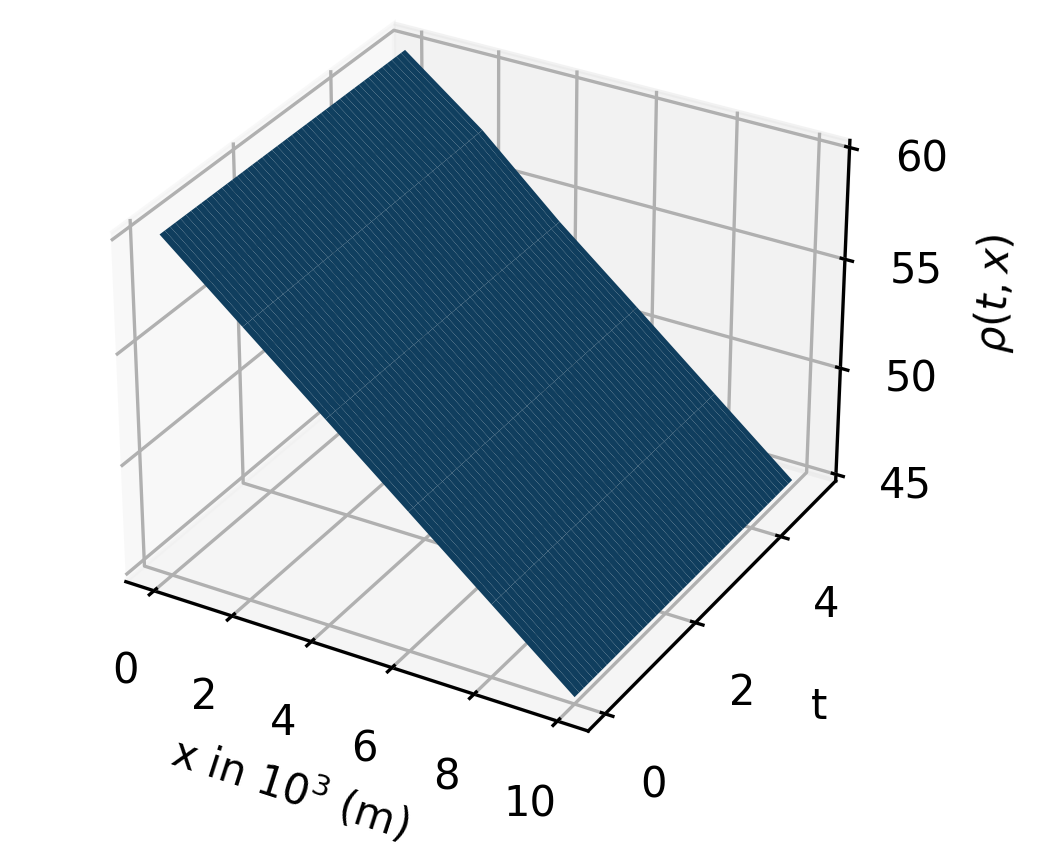
\includegraphics[height=0.3\textheight]{images/Euler_Simpl_P.png}
  &
  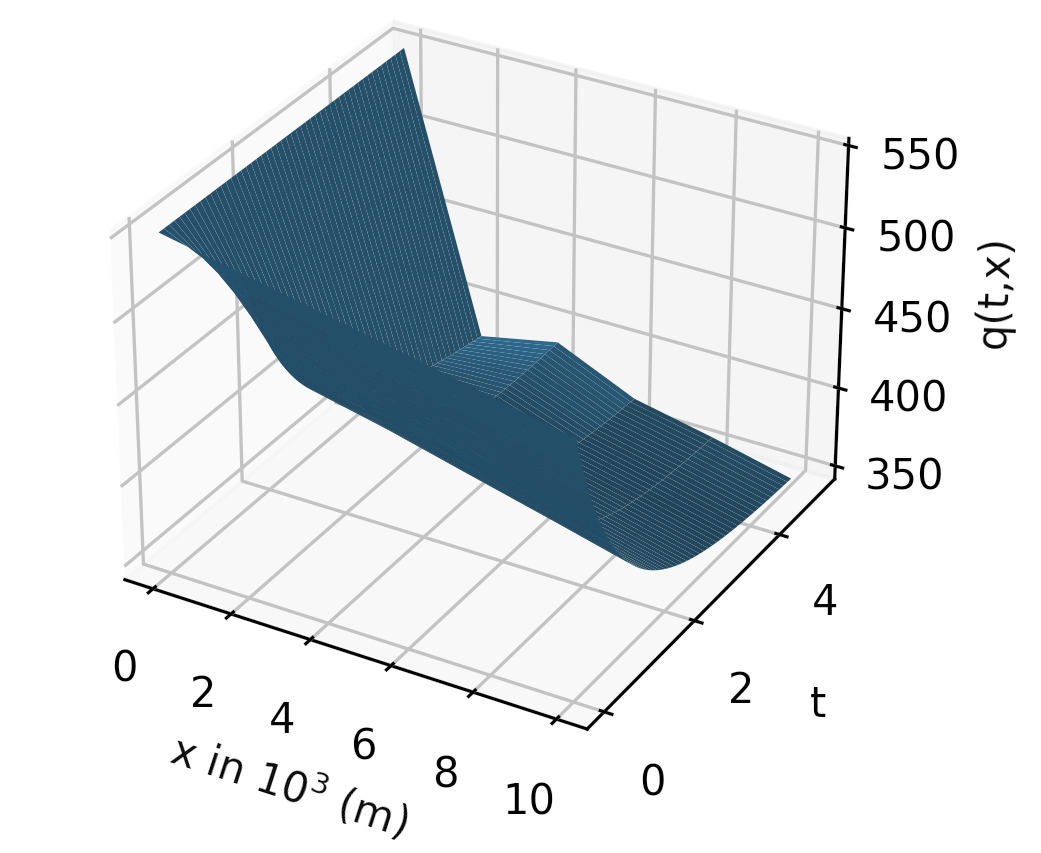
\includegraphics[height=0.3\textheight]{images/Euler_Simpl_Q_new.png}
   \\                                                     
Euler Equation: $\rho(t,x)$ & Euler Equation: $q(t,x)$
 \end{tabular}
 \begin{tabular}{cc}
  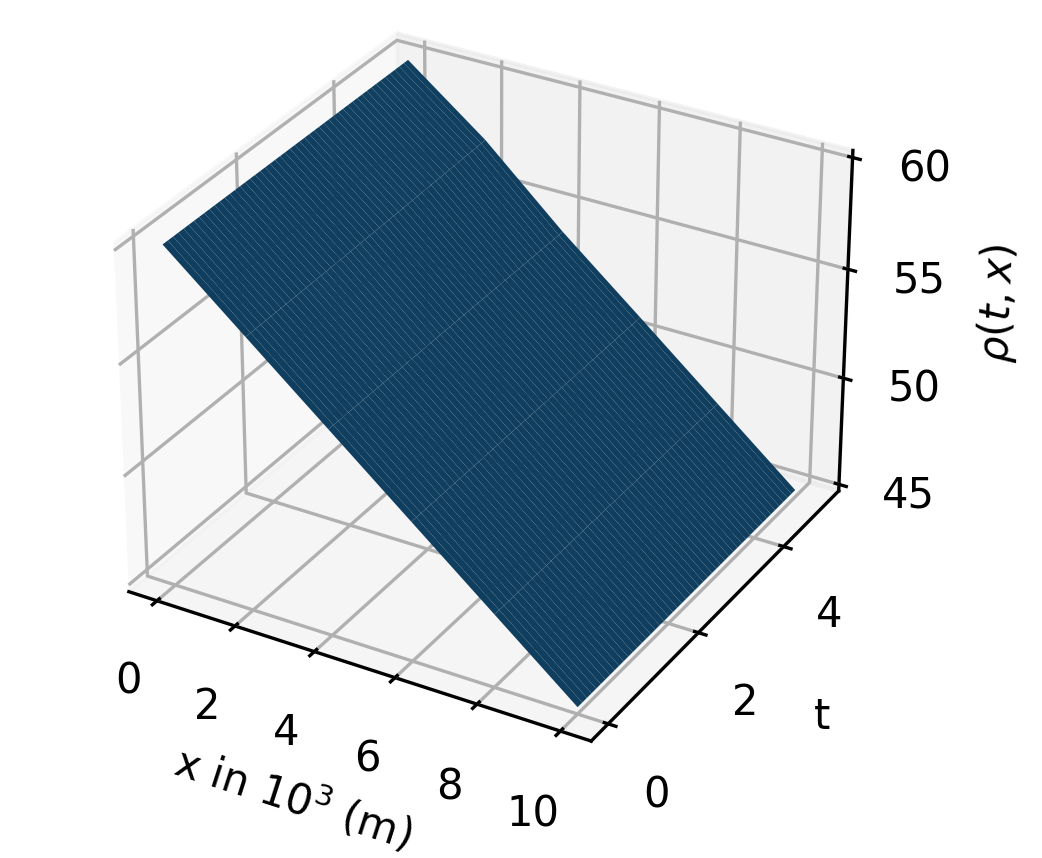
\includegraphics[height=0.3\textheight]{images/Wey_Simpl_P.png}
  &
  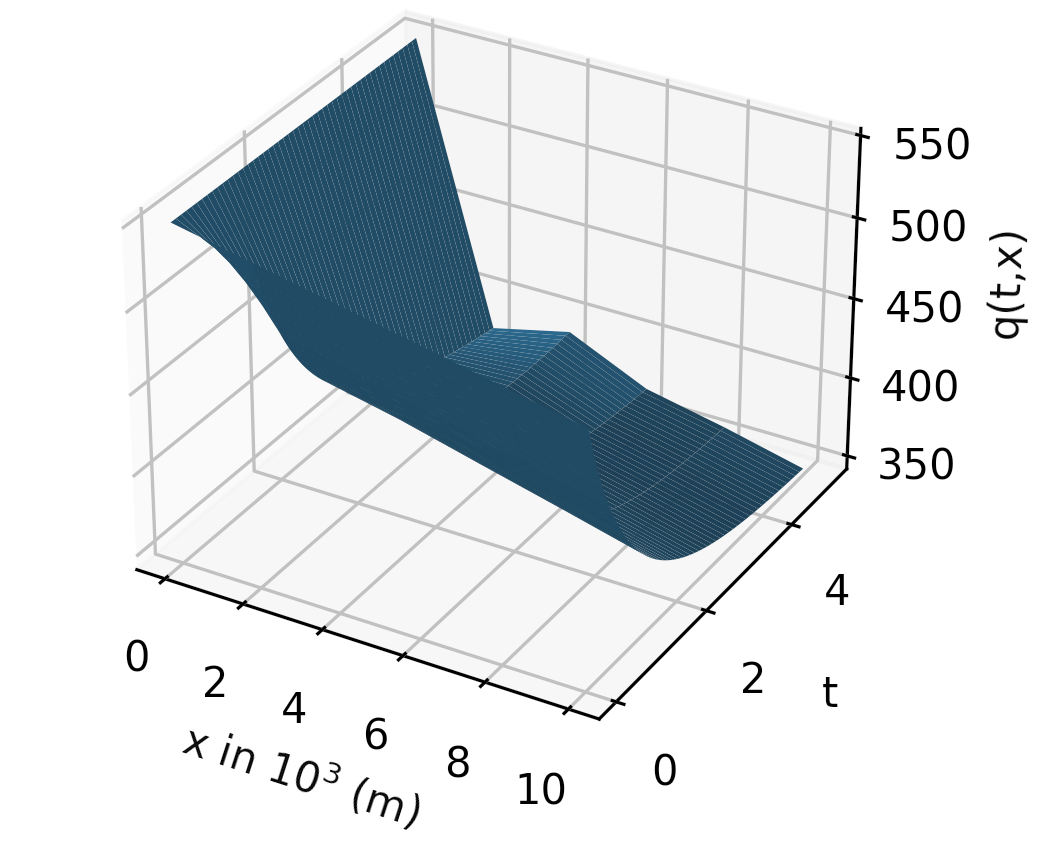
\includegraphics[height=0.3\textheight]{images/Wey_Simpl_Q_new.png}
   \\                                                     
Weymouth Equation: $\rho(t,x)$ & Weymouth Equation: $q(t,x)$
 \end{tabular}
 \end{center}
 \textcolor{bluepurp}{Note:} No difference can be spotted!
\end{frame}

\begin{frame}{Notation for Gas-Node Conditions}
$V$: set of all \textcolor{orange}{\textit{gas nodes}}\newline
$V_q$: set of all \textcolor{orange}{\textit{source nodes}} \newline
$V_p$: set of all \textcolor{orange}{\textit{sink nodes}} \newline
$V_c$: set of all \textcolor{orange}{\textit{compressor nodes}} \newline \newline
$\delta^+(v)$: set of \textcolor{orange}{\textit{outgoing edges}} at node $v \in V$ \newline
$\delta^-(v)$: set of \textcolor{orange}{\textit{ingoing edges}} at node $v \in V$ \newline\newline
${}^\text{e}q(x^n,t)$: flow in pipe $e$ in point $(x^n,t)$\newline
\textcolor{bluepurp}{Note:} Similiar for ${}^\text{e}p(x^n,t)$.
\end{frame}

\begin{frame}{Conditions at Gas Nodes (1)}
\Fontli
\textcolor{bluepurp}{Gas Coupling Conditions} \newline\newline
Sum of ingoing flows is equal to sum of outgoing flows:
\begin{equation}
\sum_{e \in \delta^-(v)}  {}^\text{e}q(x^n,t) = \sum_{h \in \delta^+(v)} {}^\text{h}q(x^0,t),  \quad  \forall v \in V \setminus (V_q \cup V_p), \; t = 0,...,T.
\end{equation}
No pressure loss near the node: \newline
For a fix but arbitrary node in the innodes $v \in V\setminus (V_q \cup V_c  \cup V_p)$ and a pressure $p(v,t)$ at node $v$ in time $t$ we state
\begin{alignat}{2}
\begin{split}
{}^\text{e}p(x^n,t) &= p(v,t), \quad \forall e \in \delta^-(v),  \;  t = 0,...,T\\
{}^\text{h}p(x^0,t) &= p(v,t), \quad \forall h \in \delta^+(v), \;  t = 0,...,T.
\end{split}
\label{Eq:5.16}
\end{alignat}
\ \newline\newline
\textcolor{bluepurp}{Gas-Power Coupling at Slack Node $s$}\newline\newline
$s$ is the gas node connected to slack bus via edge $h_{slack}$,  $\epsilon^t$ is flow taken out of the gas network.  At slack node $s$ it holds:
\begin{equation}
\sum_{e \in \delta^-(s)} {}^\text{e}q(x^n,t) = \sum_{h \in \delta^+(s)\setminus {h_{slack}}}  {}^\text{h} q(x^0,t)  + \epsilon^t, \quad t = 0,...,T.
\end{equation}
\end{frame}

\begin{frame}{Conditions at Gas-Nodes (2)}
\textcolor{bluepurp}{Compressor Conditions} \newline\newline
Conditions at Compressor Node:
\begin{equation}
{}^\text{e}p(x^n,t) = {}^\text{h}p(x^0,t) +  u_v^t, \quad \forall v \in V_c,  \, e \in \delta^-(v),  \, h \in \delta^+(v), \; t = 0,...,T
\end{equation}
where $u_v^t$ denotes pressure increase ($bar$) at compressor node $v$.  \newline

\textcolor{bluepurp}{Non-negativity constraints} \newline\newline
Pressure and pressure increase cannot be negative:
\begin{alignat}{1}
&u_{v}^t \geq 0, \quad \forall v \in V_c, \;  t = 0,...,m\\
&p_{j}^t \geq 0, \quad j=0,...,n,  \;  t=0,...,m, \; \textnormal{for all pipes}
\end{alignat}
\end{frame}

\section{Optimization Model}
\begin{frame}{Compessor Cost Optimization Problem (1)}
\Fontli
Optimization Problem with \textcolor{orange}{POC reformulation:}
\begin{alignat}{1}
\begin{split}
\min_{u}\quad & \frac{1}{2}  \sum_{t=0}^m \sum_{v \in V_c}^{} (u_v^t)^2 \\
 \text{subject to: }  & \\
\text{1.    } & \mathbf{Weymouth \; Equation \; discretized \; with \; Simple \; Upwind \; Scheme} \\
\text{2.    } &  \mathbf{gas \; coupling \; conditions} \\
\text{3.   } &  \mathbf{compressor \; conditions}  \\
& {}^\text{e}p_n^t = {}^\text{h}p_0^t +  u_v^t, \quad \forall v \in V_c,  \, e \in \delta^-(v),  \, h \in \delta^+(v), \; t = 0,...,m\\
& u_{v}^t = \sum_{s=1}^{n_{oc}} w_s^t c_{v}^s u_v^t, \quad \forall v \in V_c, \; t = 0,...,m \\
& \text{where } c_{v}^s \in \{0,1\} \text{ denotes state of compressor $v$ for configuration $s$} \\
& \sum_{s=1}^{n_{oc}} w_s^t = 1 \quad \textit{(SOS-Type1)} \\
 \text{4.    } & \mathbf{non-negativity \; constraints}  \\
 \text{5.    } &  \mathbf{gas-power \; coupling \; condition} 
\end{split}
\end{alignat}
\textbf{Initial conditions:} $p_j^0$,  $q_j^0$, $j=0,...,n$ for each pipe and $\epsilon^t$,  $t = 0,...,m$. \newline
\textbf{Solution:} $p_j^t$,  $\, q_j^t$ $\, j=0,...,n$,  $t=0,...,m$  \textnormal{for each pipe}, $u_{v}^t$, $\forall v \in V_c$ and configuration $w^t$ $\, t=0,...,m$.  \newline
\end{frame}

\begin{frame}{Compessor Cost Optimization Problem (2)}
Optimization Problem \textcolor{orange}{without POC reformulation:}
\begin{alignat}{1}
\begin{split}
\min_{u}\quad & \frac{1}{2}  \sum_{t=0}^m \sum_{v \in V_c}^{} (u_v^t)^2 \\
 \text{subject to: }  & \\
\text{1.    } & \mathbf{Weymouth \; Equation \; discretized \; with \; Simple \; Upwind \; Scheme} \\
\text{2.    } & \mathbf{gas \; coupling \; conditions} \\
\text{3.   } & \mathbf{compressor \; conditions}  \\
& {}^\text{e}p_n^t= {}^\text{h}p_0^t +  u_v^t, \quad \forall v \in V_c,  \, e \in \delta^-(v),  \, h \in \delta^+(v), \; t = 0,...,m \\
& u_{v}^t = \beta_{v}^t \cdot u_{v}^t, \quad \forall v \in V_c, \; t = 0,...,m \text{ and } \beta_{v}^t \in \{0,1\} \\
 \text{4.    } & \mathbf{non-negativity \; constraints}  \\
 \text{5.    } & \mathbf{gas-power \; coupling \; condition} 
\end{split}
\end{alignat}
\textbf{Initial conditions:} $p_j^0,  \, q_j^0$ $\, j=0,...,n$,  for each pipe and $\epsilon^t$, $\; t=0,...,m$.\newline
\textbf{Solution:} $p_j^t$,  $q_j^t$,  $\, j=0,...,n$,  $t=0,...,m$,  \textnormal{for each pipe}, $u_{v}^t$ and configuration $\beta_{v}^t$ $v \in V_c$ and $\, t=0,...,m$.  \newline
\end{frame}
\begin{frame}{Additional Constraints (1)}
\textcolor{bluepurp}{Additional Constraints: Type 1} - Compressor has to keep its state for at least a time $M_1$, $M_2$ for every compressor node $v \in V_c$.  
\begin{equation}
\sum_{e=k+1}^{k+\left\lfloor\frac{M_{1}}{\Delta t}\right\rfloor} \sum_{s=1}^{n_{oc}} c_{v}^{s} w_{s}^e\geq \sum_{s=1}^{n_{oc}} c_{v}^{s}\left\lfloor \frac{M_{1}}{\Delta t}\right\rfloor\left(-w_{s}^k+w_{s}^{k+1}\right) \quad \forall k \leq m - \left\lfloor\frac{M_{1}}{\Delta t}\right\rfloor
\label{EqAdd:6.10}
\end{equation}
\begin{equation}
\sum_{e=k+1}^{k+\left\lfloor\frac{M_{2}}{\Delta t}\right\rfloor}\left(1-\sum_{s=1}^{n_{oc}} c_{v}^{s} w_{s}^e\right) \geq \sum_{s=1}^{n_{oc}} c_{v}^{s}\left\lfloor\frac{M_{2}}{\Delta t}\right\rfloor\left(w_{s}^k-w_{s}^{k+1}\right) \quad \forall k \leq m - \left\lfloor\frac{M_{2}}{\Delta t}\right\rfloor
\label{Eq:6.11}
\end{equation}
\ \newline\newline
\textcolor{bluepurp}{Additional Constraints: Type 2} - Compressor can only switch maximum $r\in \mathbb{N}$ times.
\begin{equation}
\sum_{t=1}^m \sum_{s=1}^{n_{oc}} |w_{s}^t c_v^s - w_{s}^{t-1} c_v^s | \leq r, \quad \forall v \in V_c.
\label{Eq:6.11b}
\end{equation}
\end{frame}
\begin{frame}{Additional Constraints (2)}
\textcolor{bluepurp}{Solve CIAP by solving MILP}
\begin{alignat}{1}
\begin{split}
\min_{\substack{\beta^t \in H \cap \{0,1\}^{n_{oc}},  \\ t =0,...,m-1,  \\ \delta^0 \in \mathbb{R}^{n_{oc}}, \epsilon \in \mathbb{R}}}  &\epsilon      \\
\text{subject to: } \quad &\norm{\delta^0 + \sum_{t=0}^{k-1} \Delta t (\alpha^t-w^t)}_{\Omega} \leq \epsilon \quad  \text{for all } k=0,...,m \\
& + \textcolor{orange}{additional \; constraints \; type \; 1 \, }  \text{ OR } + \textcolor{orange}{additional \; constraints \; type \; 2}
\end{split}
\label{Eq:CIAP_MILP}
\end{alignat}
where $\alpha^t$ are the relaxed binary variables in time $t$.
\end{frame}

\section{Numerical Analysis}
\begin{frame}{Algorithms used}
\Fontli
\begin{tabular}{ ll m{2.7cm} m{2cm}}\toprule
 & \textcolor{bluepurp}{Method} & \textcolor{bluepurp}{Solver} & \textcolor{bluepurp}{Programming Language}\\
 \hline
 \rule{0pt}{3ex}
Power Model & Levenberg-Marquardt & \textit{fsolve} & Matlab\\
\rule{0pt}{5ex}
Three-Step Approach & Interior Point Method & IPOPT 3.12.3 with ma27 integrated in CasADi& Python 3.7.6\\
& ($+$ Sum Up Rounding  & & \\
& or MILP) & Gurobi 9.1.2 & \\ \rule{0pt}{5ex}
Direct Solver & NLP-Based& BONMIN integrated in CasADi & Python 3.7.6\\
& Branch-and-Bound &  & \\
& Algorithm &  & \\
\bottomrule
\end{tabular}
\newline\newline\newline\newline
\textcolor{bluepurp}{PC}: MacBook Pro,  16 GB RAM, Intel-Quad Core i5, \, 2,4 GHz CPU
\end{frame}

\begin{frame}{Numerical Analysis: Simple Gas Network}
\begin{figure}[l]
\centering
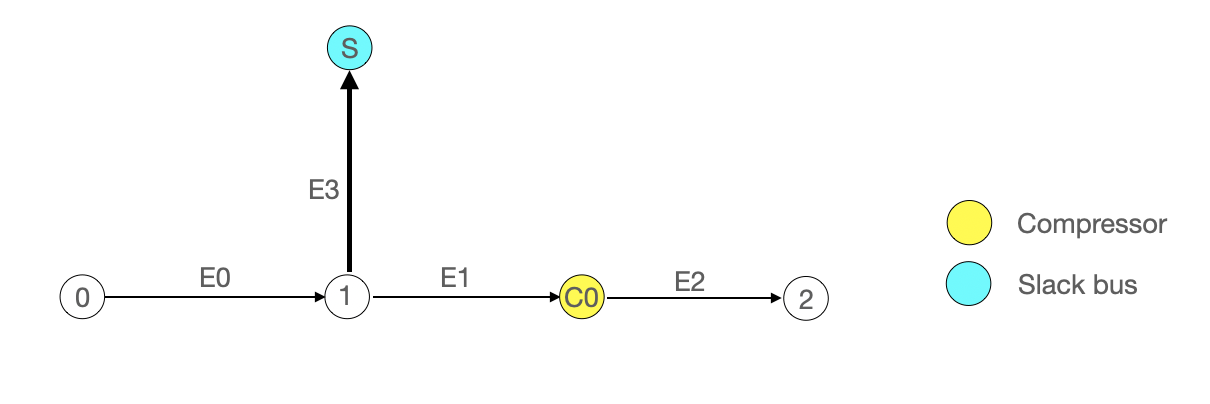
\includegraphics[width=0.6\textwidth]{images/SimpleNetwork}
\caption{Simple Model}
\label{PowerGrid}
\end{figure}
\textcolor{bluepurp}{Constants:} $\lambda = 0.11$, $D=1 \, m$ and $c = 340 \, m/s$,  pipe of length $12 \, km$,  total execution time of $5 \, sec$,  spacial step size  $\Delta x = 2000$,  time step size $\Delta t = 1/60$ \newline\newline
\textcolor{bluepurp}{Initial data:} $\epsilon^t=0,$ $t=0,...,m$,  $p(0,x)= 60 \, bar$ and $q(0,x) = 500 \, kg/s$ for each pipe at every pipe section
\end{frame}

\begin{frame}{Numerical Analysis: Simple Model}
\begin{tabular}{ccc} \hline
Bonmin (no POC)& Bonmin (POC) & Three-Step Approach \\\hline
 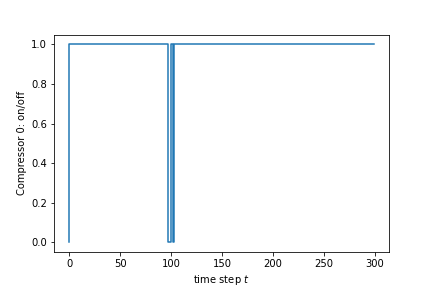
\includegraphics[width=.32\textwidth]{images/bonmin_control_beta.png} &   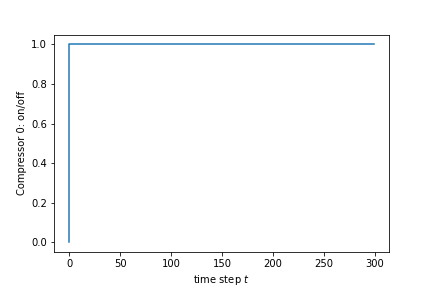
\includegraphics[width=.32\textwidth]{images/BONMINConf.png} & 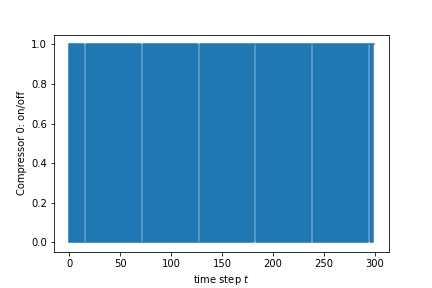
\includegraphics[width=.32\textwidth]{images/POCConf.png}  \\ 
  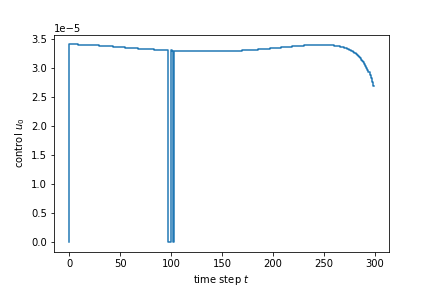
\includegraphics[width=.32\textwidth]{images/bonmin_control_u.png} &   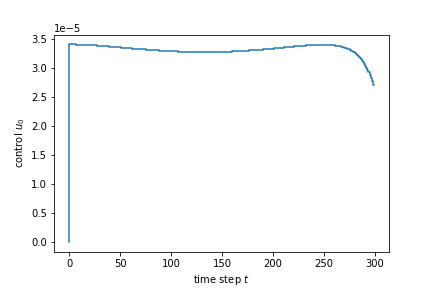
\includegraphics[width=.32\textwidth]{images/BONMINControl_u.png} & 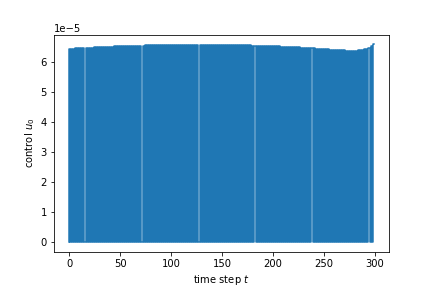
\includegraphics[width=.32\textwidth]{images/POCControl_u.png}  \\ 
\textcolor{orange}{OFV:} $1.6350264 \cdot 10^{-7}$ & \textcolor{orange}{OFV:}  $1.64764 \cdot 10^{-7}$  & \textcolor{orange}{OFV:}  $3.1675 \cdot 10^{-7}$ \\ 
\textcolor{orange}{Runtime:} 107.35 $sec$ & \textcolor{orange}{Runtime:}  176.13 $sec$ & \textcolor{orange}{Runtime:}  7.59 $sec$ \\
($\approx 1.8 \, min$) & ($\approx 2.9 \, min$) &
\end{tabular} 
\end{frame}

\begin{frame}{Additional Constraints: Simple Model}
\framesubtitle{Three-Step Approach with and without Additional Constraints}
\begin{tabular}{c p{3cm} p{3cm}} \hline
No Add.Constraints & Add. Constraint Type 1& Add. Constraint Type 2 \\\hline
& Compressor can only switch $5$ times in $5 \, sec $& Compressor has to keep its state for at least $3$ time steps \\
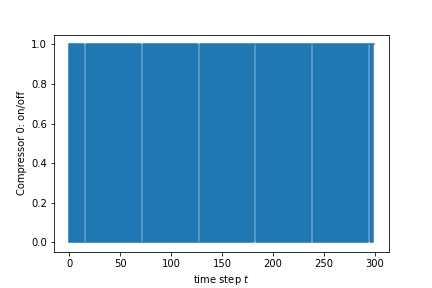
\includegraphics[width=.32\textwidth]{images/POCConf.png}  &   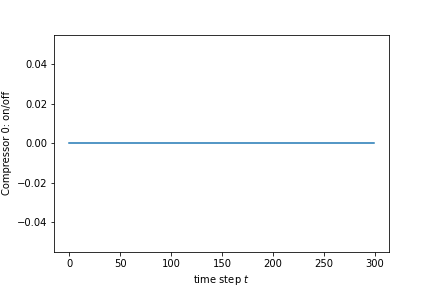
\includegraphics[width=.32\textwidth]{images/AC_Simple/POCConf.jpg} & 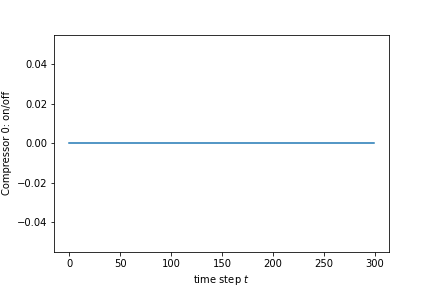
\includegraphics[width=.32\textwidth]{images/AC_Simple/POCConf.jpg}  \\ 
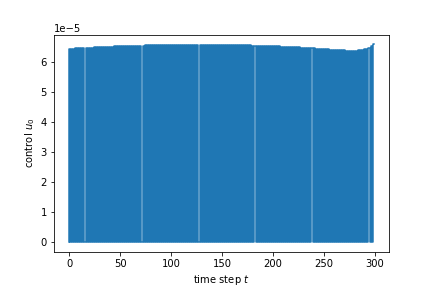
\includegraphics[width=.32\textwidth]{images/POCControl_u.png} &   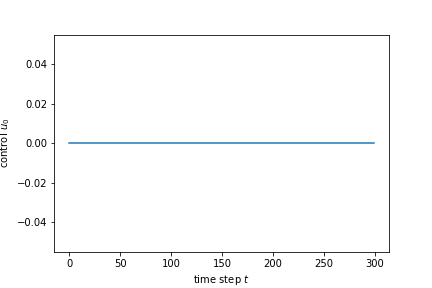
\includegraphics[width=.32\textwidth]{images/AC_Simple/POCControl_u.jpg}  & 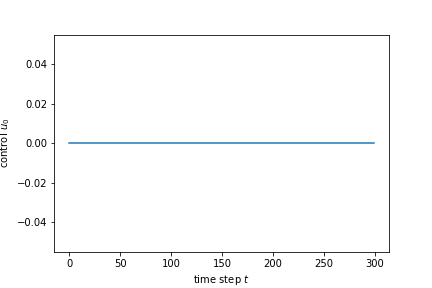
\includegraphics[width=.32\textwidth]{images/AC_Simple/POCControl_u.jpg}    \\ 
\textcolor{orange}{OFV:} $3.1675 \cdot 10^{-7}$ & \textcolor{orange}{OFV:}  $1.5 \cdot 10^{-14}$  & \textcolor{orange}{OFV:}  $1.5 \cdot 10^{-14}$ \\ 
\textcolor{orange}{Runtime:} 7.59 $sec$ & \textcolor{orange}{Runtime:}  12.41 $sec$  & \textcolor{orange}{Runtime:}  18.21 $sec$ \\
\end{tabular}
\end{frame}

\begin{frame}{Numerical Analysis: Advanced Model}
\Fontli
\begin{tabular}{cc}
  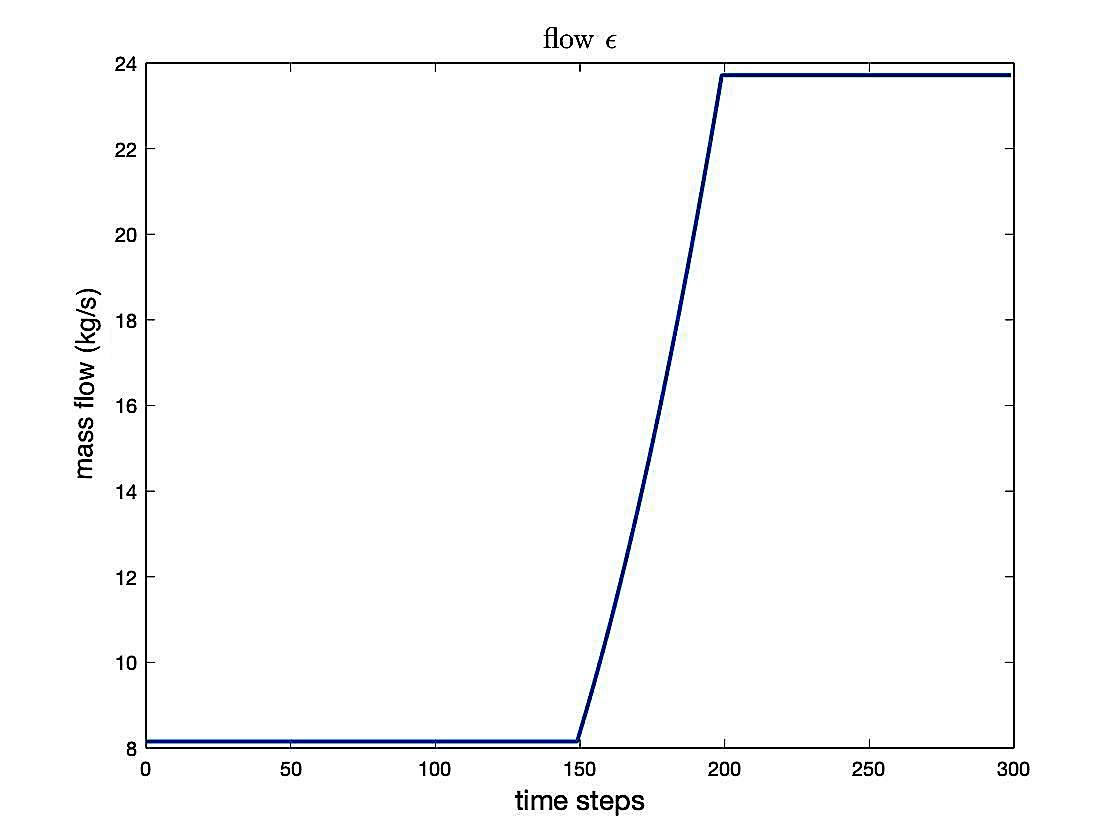
\includegraphics[height=0.4\textheight]{images/eps_advanced_new.jpg}& 
  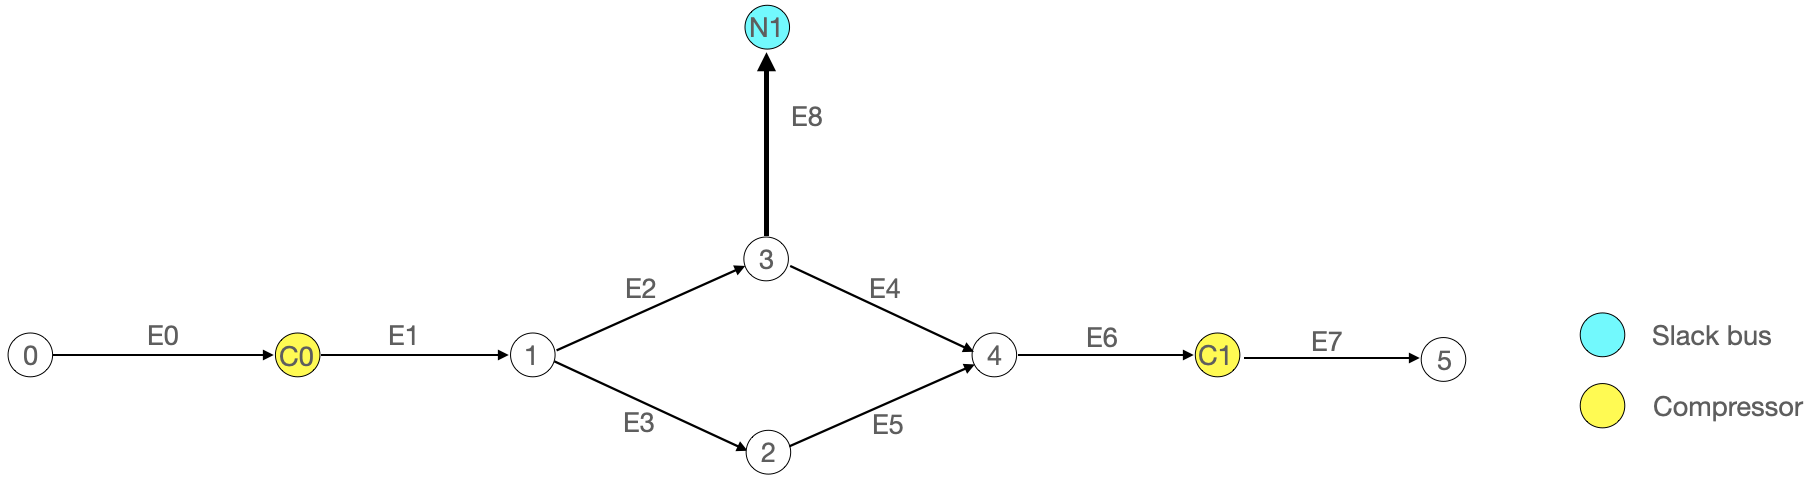
\includegraphics[height=0.18\textheight]{images/AdvancedNetwork} 
   \\                                                     
\textcolor{bluepurp}{Figure 8} & Advanced Gas Network 
 \end{tabular}
 \ \newline\newline
\textcolor{bluepurp}{Constants:} $\lambda = 0.11$, $D=1 \, m$ and $c = 340 \, m/s$,  pipe of length $12 \, km$,  total execution time of $5 \, sec$, spacial step size  $\Delta x = 2000$,  time step size $\Delta t = 1/60$  \newline\newline
\textcolor{bluepurp}{Initial data:} \newline\newline
\begin{tabular}{lllllllll}\toprule
& $E0$ &$E1$ & $E2,\, E3$ &$E4$ &$E5$&$E6, \, E7$\\
 \hline
$p(x,0) \, (bar)$ & $60$ & $62$ & $62$ & $62$ &$62$ &$62$ \\
$q(x,0) \, (kg/s)$ & $500$ & $500$ & $250$ & $241.847$ &$250$ &$491.847$\\
\bottomrule
\end{tabular}
\newline\newline\newline
$\epsilon^t $ (mass taken out of gas network is shown in \textcolor{bluepurp}{Figure 8})
\end{frame}

\begin{frame}{Numerical Analysis: Advanced Model}
\begin{columns}[T]
\begin{column}{.48\textwidth}
\begin{tabular}{c} \hline
Three-Step Approach \\\hline
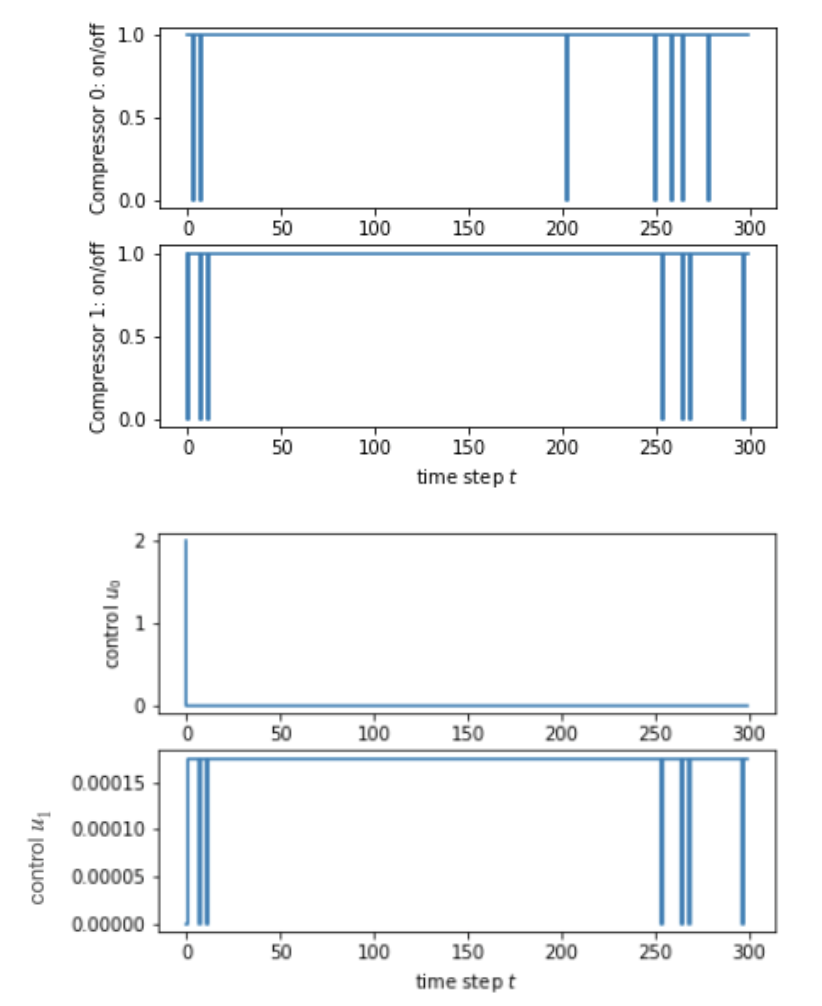
\includegraphics[width=0.9\textwidth]{images/AdvancedModel3Step} \\
\textcolor{orange}{OFV:} $2.00000$  \\ 
\textcolor{orange}{Runtime:} 1259.03 $sec$ ($\approx$ 21 $min$)
\end{tabular}
\end{column}
\begin{column}{.48\textwidth}
\begin{center}
\begin{itemize}
\item solved to 'acceptable level' (tolerance level $10^{-6}$)
\item direct solver bonmin could not find any result in $2 \, hours$ - freezing behaviour.  
\end{itemize}
\end{center}
\end{column}
\end{columns}
\end{frame}

\begin{frame}{Additional Constraints: Advanced Model}
\framesubtitle{Three-Step Approach with and without Additional Constraints}
\begin{tabular}{l p{3cm} p{3cm}} \hline
No Add.Constraints & Add. Constraint Type 1& Add. Constraint Type 2 \\\hline
& Compressor can only switch $10$ times in $5 \, sec $& Compressor has to keep its state for at least $3$ time steps \\
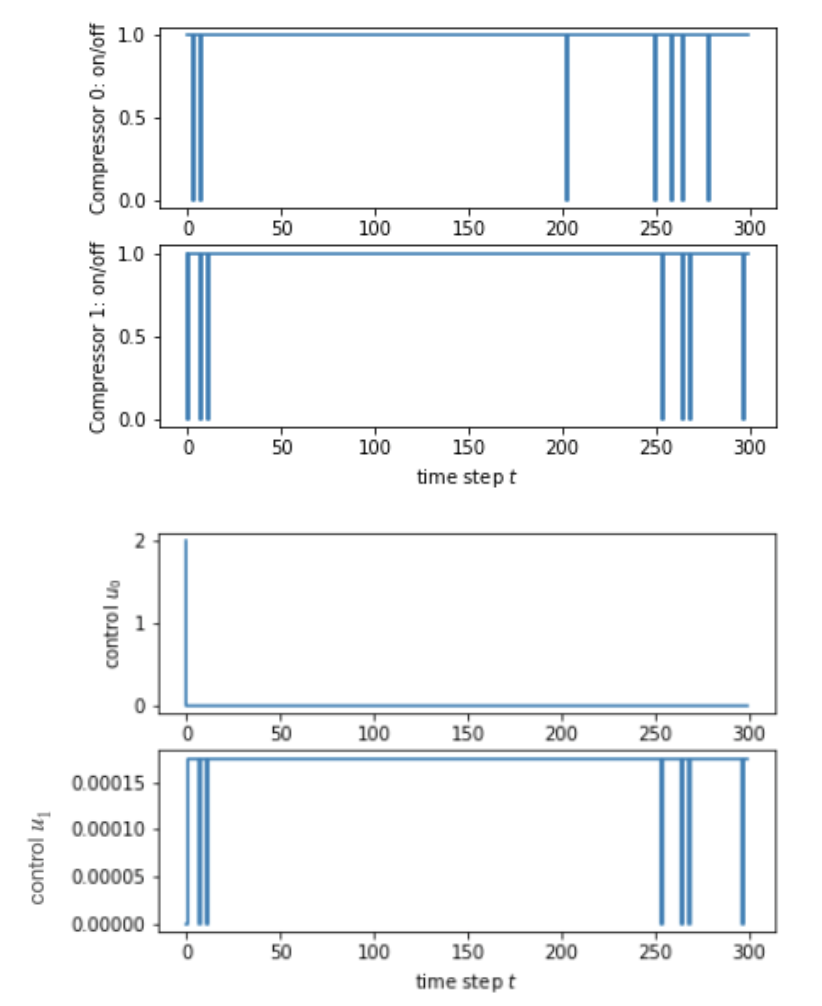
\includegraphics[width=.32\textwidth]{images/AdvancedModel3Step} & 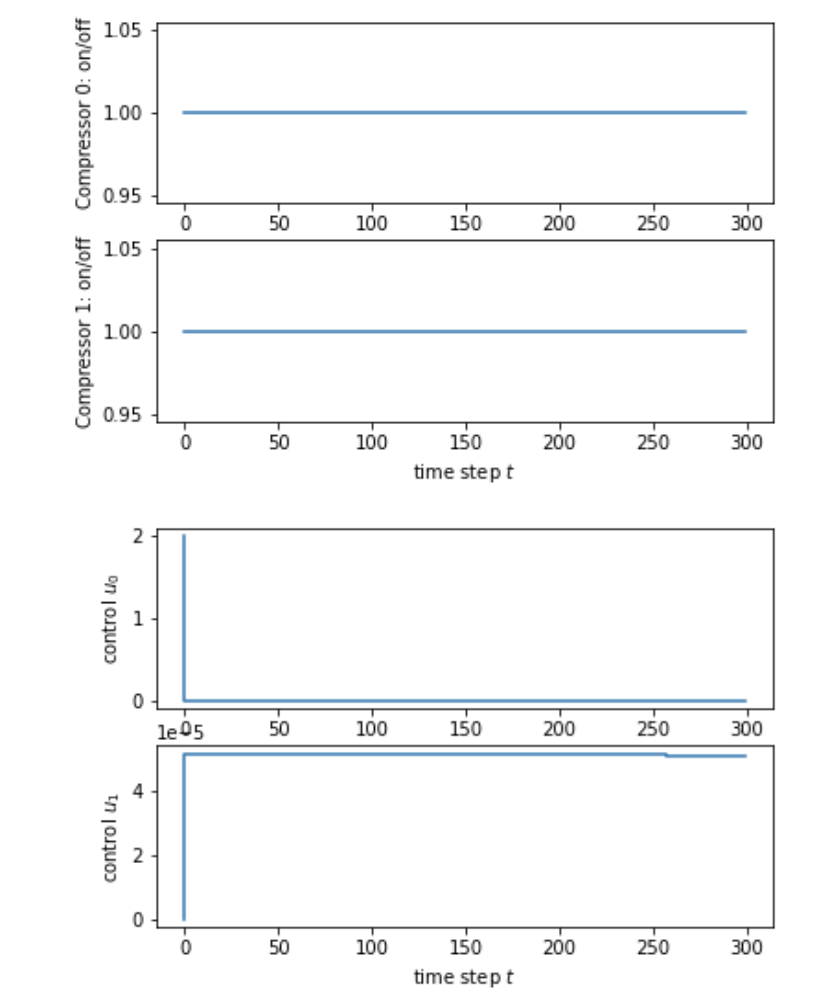
\includegraphics[width=.32\textwidth]{images/AdvancedModel3Step2}& 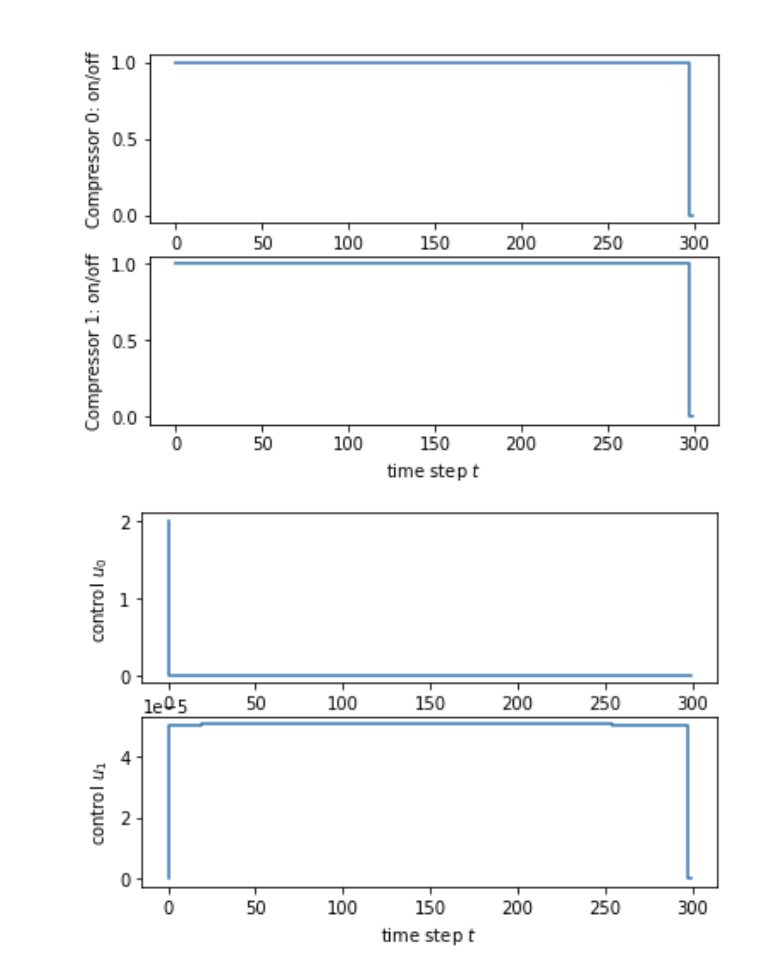
\includegraphics[width=.32\textwidth]{images/AdvancedModel3Step3}   \\
\textcolor{orange}{OFV:} $2.0000$ & \textcolor{orange}{OFV:}  $2.0000$ & \textcolor{orange}{OFV:}  $2.0000$ \\ 
\textcolor{orange}{Runtime:} 1259 $sec$ ($\approx$ 21 $min$) & \textcolor{orange}{Runtime:}  1941.63 $sec$ ($\approx$ 32.3 $min$) & \textcolor{orange}{Runtime:}  1920.15 $sec$ ($\approx$ 32 $min$)\\
\end{tabular}
\end{frame}

\section{Conclusion}
\begin{frame}{Conclusion}
\begin{itemize}
\item Three Step Approach delivers good optimization results and is up to \textcolor{orange}{14 times} faster than direct solver bonmin, which works with the NLP-based Brand-and-Bound algorithm
\item With additional constraints we can prevent the compressor from \textcolor{orange}{switching too often} and can achieve even better OFV
\item Due to the CFL Condition we had to choose a very small time step ($\Delta t = \frac{1}{60}$) and therefore considered a simulation of $5 \,  sec$.  For realistic simulations (e.g. 1 day) computation will likely take several hours.  \newline
Interesting question: How does run time and solutions vary for \textcolor{orange}{implicit scheme} and \textcolor{orange}{explicit scheme} (with Three Step approach)?
\end{itemize}
\end{frame}

\begin{frame}
\begin{center}
Thank you for your attention!
\end{center}
\end{frame}

\end{document}